%!TEX root=../GaugeCNNTheory.tex


\subsubsection*{هموردایی دورانی سراسری روی $\Euc_3 \backslash \{0\}$}
\label{sec:punctured_euclidean_3dim}

ایده‌های ارائه شده در بالا را می‌توان به محیط سه‌بعدی، یعنی به فضای اقلیدسی سوراخ‌دار $\Euc_3 \backslash \{0\}$ تعمیم داد.
کانولوشن‌های $\GM$ هموردای دورانی سراسری در اینجا متناظر با $G$-ساختارهایی هستند که تحت دوران‌های $\SO3$ حول مبدأ ناوردا هستند.
در حالی که وابستگی شعاعی چنین $G$-ساختارهایی بدون محدودیت باقی می‌ماند، تقاضا برای ناوردایی دورانی، محدودیتی را بر شکل آنها روی پوسته‌های کروی با شعاع ثابت، که مدارهای عمل~$\SO3$ روی $\Euc_3 \backslash \{0\}$ هستند، تحمیل می‌کند.
این واقعیت که کره $S^2 = \SO3/\SO2$ یک فضای همگن از $\SO3$ با زیرگروه‌های پایدارساز ایزومورف با $\SO2$ است، دلالت بر این دارد که گروه ساختاری یک $G$-ساختار $\SO3$-ناوردا را نمی‌توان بیشتر از $G=\SO2$ کاهش داد؛ به شکل~\ref{fig:G_structure_S2_1} مراجعه کنید.
بنابراین ما اساساً با \lr{CNN}های کروی با یک بعد شعاعی اضافی سروکار داریم.
برای مروری بر \lr{CNN}های کروی، خواننده را به بخش~\ref{sec:instantiations_spherical} ارجاع می‌دهیم.


\citet{ramasinghe2019representation} این وضعیت را شناسایی کرده و کانولوشن‌های $\SO3$-هموردا را روی $\Euc_3 \backslash \{0\}$ طراحی کردند.
قبل از پرداختن به طبقه‌بندی ما به عنوان کانولوشن $\GM$ که در ردیف (۲۹) جدول~\ref{tab:network_instantiations} فهرست شده است، به طور خلاصه فرمول‌بندی و پیاده‌سازی نویسندگان را مرور می‌کنیم.
پیاده‌سازی آنها مبتنی بر \lr{CNN}های کروی است با این اضافه که
۱) کرنل‌ها در جهت شعاعی گسترش می‌یابند و
۲) روی پوسته‌هایی با شعاع‌های مختلف به اشتراک گذاشته می‌شوند؛ به شکل~\ref{fig:G_structure_R3_no_origin} (چپ) مراجعه کنید.
همانطور که معمولاً برای \lr{CNN}های کروی انجام می‌شود، وابستگی زاویه‌ای کرنل‌ها از طریق طیف فوریه آنها روی~$S^2$ کدگذاری می‌شود، یعنی بر حسب ضرایب بسط هارمونیک‌های کروی.
اشتراک این ضرایب بسط دلالت بر این دارد که کرنل‌های به اشتراک گذاشته شده زاویه فضایی یکسانی را برای همه شعاع‌ها پوشش می‌دهند، که به این معنی است که \emph{کرنل‌ها در جهت زاویه‌ای به صورت خطی با شعاع گشاد می‌شوند}.%
\footnote{
	گشادی در اینجا نسبت به متریک اقلیدسی استاندارد $\Euc_3 \backslash \{0\}$ اندازه‌گیری می‌شود.
}
در پیاده‌سازی گسسته‌سازی شده، پوسته‌های کروی در شعاع‌های با فاصله مساوی قرار دارند -- که این به معنی آن است که \emph{کرنل‌ها در جهت شعاعی گشاد نمی‌شوند}.
از این بینش‌ها، ما $G$-ساختار خاصی را که مدل در ادامه فرض می‌کند، استنباط می‌کنیم.
خود کرنل‌ها به گونه‌ای محدود شده‌اند که تحت دوران‌های $\SO2$ حول محور شعاعی گذرنده از مرکزشان ناوردا باشند، که اغلب به آن \emph{کرنل‌های ناحیه‌ای (zonal)} گفته می‌شود؛
به شکل~\ref{fig:zonal_kernel} و~\cite{esteves2018zonalSpherical} مراجعه کنید.
همانطور که در~\cite{esteves2018zonalSpherical} و~\cite{ramasinghe2019representation} اثبات شده است، کانولوشن با چنین کرنل‌هایی $\SO3$-هموردا است.
اینکه این مورد برقرار است، به طور شهودی روشن است زیرا دوران‌های پوسته‌های کروی دارای $\SO2$ به عنوان زیرگروه پایدارساز هستند، که کرنل‌های ناحیه‌ای نسبت به آن ناوردا هستند.
همانطور که در ادامه استدلال خواهیم کرد، این مدل در واقع $\OO3$-هموردا است، یعنی علاوه بر آن تحت بازتاب‌ها نیز هموردا است.

\begin{figure}
	\centering
	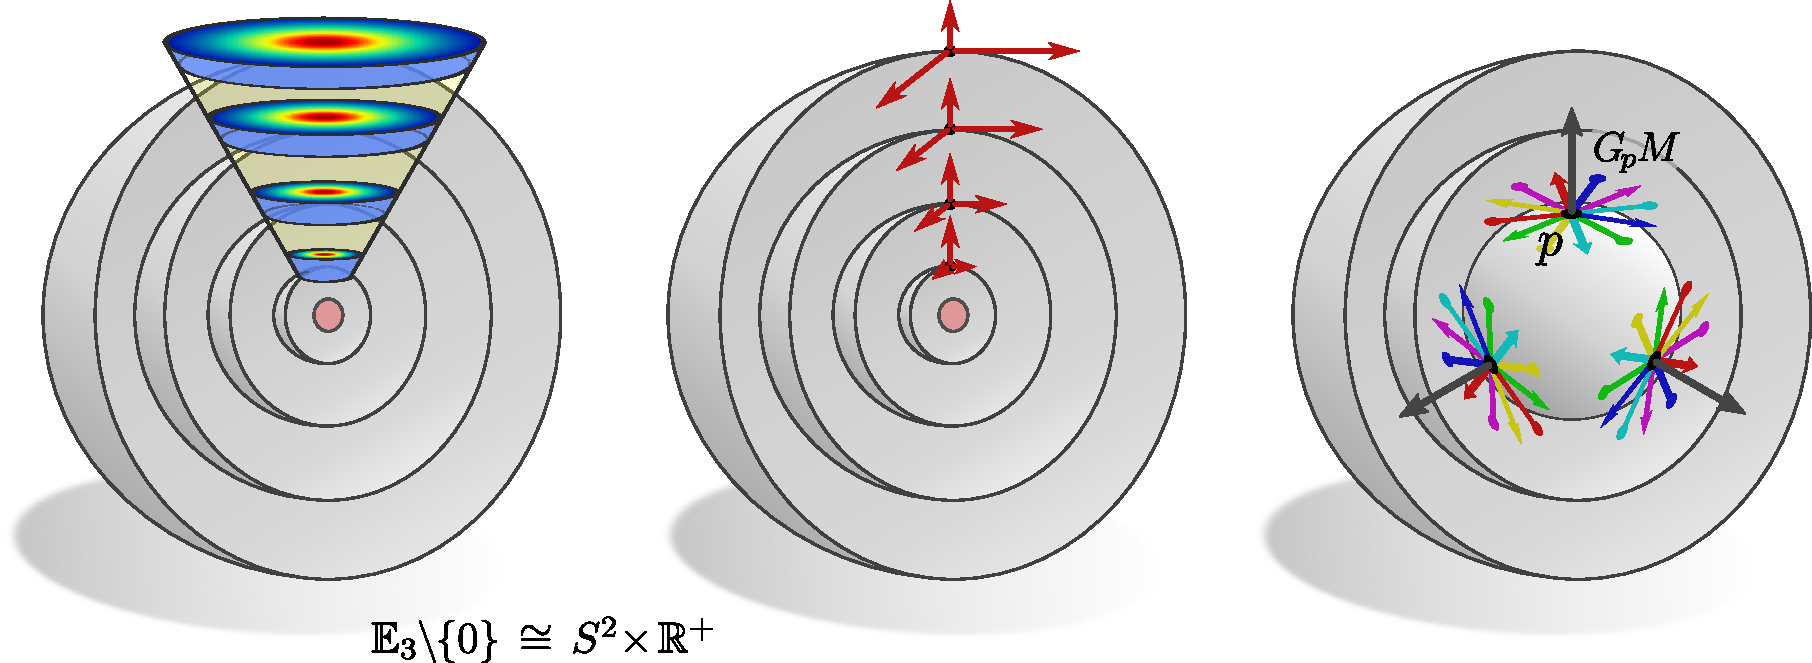
\includegraphics[width=1.\textwidth]{figures/G_structure_R3_no_origin.pdf}
	\hfill
	\caption{\small
		$G$-ساختاری که به طور ضمنی توسط~\citet{ramasinghe2019representation} فرض شده بود را می‌توان از طرح اشتراک وزن استنتاج کرد.
		\emph{چپ:}
		اشتراک وزن کرنل‌های کانولوشن (همسانگرد) روی $\Euc_3 \backslash \{0\} \cong S^2 \times \R^+$ همانطور که در~\cite{ramasinghe2019representation} پیشنهاد شده است.
		کرنل‌ها به گونه‌ای تعریف شده‌اند که زاویه فضایی یکسانی را پوشش دهند، مستقل از فاصله از مبدأ، به طوری که قطر آنها به صورت خطی با این فاصله رشد می‌کند.
		گستره کرنل‌ها در جهت شعاعی مستقل از فاصله از مبدأ است.
		\emph{وسط:}
		در نظریه ما، کرنل‌ها نسبت به چارچوب‌های مرجع از $G$-ساختار به اشتراک گذاشته می‌شوند.
		برای بازیابی طرح اشتراک وزن پیشنهادی، $\GM$ باید از چارچوب‌هایی تشکیل شود که محورهای آنها در جهت زاویه‌ای به صورت خطی با فاصله شعاعی از مبدأ رشد می‌کنند، در حالی که محورها در جهات شعاعی باید اندازه خود را ثابت نگه دارند (هر دو نسبت به متریک اقلیدسی استاندارد).
		چنین چارچوب‌هایی یک متریک ریمانی جایگزین را روی $\Euc_3 \backslash \{0\}$ القا می‌کنند.
		\emph{راست:}
		از آنجا که کانولوشن $\GM$ حاصل باید $\SO3$-هموردا باشد، لازم است که $G$-ساختار تحت دوران حول مبدأ ناوردا باشد.
		این امر (حداقل) به یک $\SO2$-ساختار نیاز دارد، که تحدید آن به یک پوسته کروی در قسمت سمت راست شکل نشان داده شده است.
		این را با $\SO2$-ساختار $\SO3$-ناوردای \lr{CNN}های کروی در شکل~\ref{fig:G_structure_S2_1} مقایسه کنید.
	}
	\label{fig:G_structure_R3_no_origin}
\end{figure}


\begin{wrapfigure}[13]{r}{0.25\textwidth}
	\vspace*{-3.ex}
	\centering
	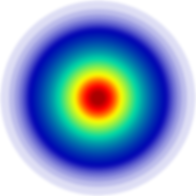
\includegraphics[width=.8\linewidth]{figures/invariant_kernel.png}%
	\caption{\small
		یک کرنل \emph{ناحیه‌ای} (همسانگرد) به طور همزمان $\SO2$- و $\OO2$-راهبری‌پذیر است؛
		معادلات~\eqref{eq:Euc3_punctured_SO2_constraint} و~\eqref{eq:Euc3_punctured_O2_constraint} را مقایسه کنید.
	}
	\label{fig:zonal_kernel}
\end{wrapfigure}%
برای بازیابی این مدل از دیدگاه کانولوشن‌های $\GM$، ما باید $G$-ساختار متناظر را روی $M = \Euc_3 \backslash \{0\}$ تعیین کنیم.
همانطور که در بالا گفته شد، هموردایی $\SO3$ مدل نیازمند این است که $G$-ساختار تحت عمل $\SO3$ ناوردا باشد اما تغییرات شعاعی آن را محدود نمی‌کند.
برای استنتاج این وابستگی شعاعی $G$-ساختار، به یاد بیاورید که ما اشتراک وزن کانولوشنی را در $p\in M$ به عنوان تراز کردن کرنل الگو $K: \R^3 \to \R^{\cout\times\cin}$ نسبت به یک چارچوب (دلخواه) در $\GpM$ از فضاهای مماس $\TpM$ تعریف کردیم.
بنابراین، اشتراک کرنل در نظر گرفته شده توسط \citet{ramasinghe2019representation} به ما اجازه می‌دهد تا در مورد $G$-ساختار به طور ضمنی در نظر گرفته شده نتیجه‌گیری کنیم.
نویسندگان کرنل‌ها را به گونه‌ای به اشتراک می‌گذارند که مساحت مماس آنها بر پوسته‌های کروی با افزایش فاصله از مبدأ گسترش یابد (آنها زاویه فضایی یکسانی را در هر شعاع پوشش می‌دهند) در حالی که ضخامت شعاعی آنها ثابت باقی می‌ماند.
شکل~\ref{fig:G_structure_R3_no_origin} (چپ) این تغییر شعاعی کرنل‌های به اشتراک گذاشته شده را نشان می‌دهد در حالی که
شکل~\ref{fig:G_structure_R3_no_origin} (وسط) مقیاس‌بندی متناظر چارچوب‌های مرجع نمونه را نشان می‌دهد.
این به همراه ناوردایی $\SO3$ مورد نیاز $G$-ساختار، (حداقل) یک $\SO2$-ساختار را نتیجه می‌دهد، که تحدید آن به یک پوسته کروی در شکل~\ref{fig:G_structure_R3_no_origin} (راست) به تصویر کشیده شده است.%
\footnote{
	مشابه دوبعدی آن شبیه به $G$-ساختار در شکل~\ref{fig:G_structure_R2_no_origin_logpolar} خواهد بود اما با تمام بردارهای چارچوب در جهت شعاعی که دارای نرم واحد هستند (نسبت به متریک اقلیدسی).
}
متریک در نظر گرفته شده از این $G$-ساختار نتیجه می‌شود، زیرا چارچوب‌های آن مفهوم مربوط به راست‌هنجاری را تعریف می‌کنند.
توجه داشته باشید که این متریک با متریک اقلیدسی معمول متفاوت است.


بنا به ساختار، ما دوران‌های $\IsomGM = \SO3$ را به عنوان ایزومتری‌های حافظ $G$-ساختار داریم.
بنابراین، کانولوشن‌های $\GM$ تعریف شده توسط این $G$-ساختار، که ممکن است در نوع میدان ورودی و خروجی خود متفاوت باشند، (طبق قضیه~\ref{thm:isom_equiv_GM_conv}) هموردای دورانی خواهند بود.
کانولوشن $\GM$ خاصی که توسط \citet{ramasinghe2019representation} فرض شده، یعنی انواع میدان فرض شده، را می‌توان از این واقعیت استنتاج کرد که نویسندگان کرنل‌های ناحیه‌ای را فرض می‌کنند:
چنین کرنل‌هایی به طور طبیعی هنگام در نظر گرفتن \emph{میدان‌های اسکالر}، یعنی نمایش‌های میدان بدیهی، به وجود می‌آیند، زیرا محدودیت کرنل، معادله~\eqref{eq:kernel_constraint}، در این حالت به صورت زیر در می‌آید
\begin{align}\label{eq:Euc3_punctured_SO2_constraint}
	K(g\mkern1mu \mathscr{v}) = K(\mathscr{v}) \quad\ \forall\ \mathscr{v}\in\R^3,\ g\in\SO2 \,,
\end{align}
که کرنل‌های همسانگرد (ناحیه‌ای) را تحمیل می‌کند.%
\footnote{
	کرنل‌هایی که بین «میدان‌های اسکالر»، یعنی میدان‌هایی که مطابق با نمایش بدیهی~$G$ تبدیل می‌شوند، نگاشت انجام می‌دهند، همیشه $G$-ناوردا هستند.
	برای $G=\SO2$ این به معنی کرنل‌های همسانگرد (ناحیه‌ای) است، در حالی که $G=\Flip$ به معنی کرنل‌های ناوردای بازتابی در ورودی بالا سمت چپ جدول~\ref{tab:reflection_steerable_kernels} است.
}


به عنوان یک تنوع از مدل، می‌توان $\OO2$-ساختار را در نظر گرفت که از $\SO2$-ساختار با افزودن چارچوب‌های مرجع بازتابیده (بازتاب نسبت به یک محور دلخواه در داخل صفحات مماس بر پوسته‌های کروی، در حالی که بردارهای چارچوب شعاعی همچنان به سمت بیرون اشاره دارند) به دست می‌آید.%
\footnote{
	این $\OO2$-ساختار، همتای $\OO1 = \Flip$-ساختار در شکل~\ref{fig:G_structure_R2_no_origin_O2} برای $d=3$ به جای $d=2$ است.
}
در این حالت، ایزومتری‌های حافظ $G$-ساختار $\IsomGM = \OO3$ وجود دارند که از دوران‌ها و بازتاب‌های سراسری حول مبدأ تشکیل شده‌اند و بنابراین کانولوشن‌های $\GM$ هموردای $\OO3$ هستند.
یک مورد خاص جالب در زمینه فعلی، کانولوشن‌های $\GM$ است که بین میدان‌های اسکالر نگاشت انجام می‌دهند، که برای آنها محدودیت کرنل به صورت زیر است:
\begin{align}\label{eq:Euc3_punctured_O2_constraint}
	K(g\mkern1mu \mathscr{v}) = K(\mathscr{v}) \quad\ \forall\ \ \mathscr{v}\in\R^3,\ g\in\OO2 \,.
\end{align}
این به نظر می‌رسد یک محدودیت قوی‌تر از محدودیت در معادله~\eqref{eq:Euc3_punctured_SO2_constraint} بالا باشد:
به جای اینکه فقط کرنل‌ها را ناوردای دورانی بخواهد، علاوه بر آن از آنها می‌خواهد که تحت بازتاب‌ها نیز ناوردا باشند.
با این حال، از آنجا که کرنل‌های ناوردای دورانی در حال حاضر تحت بازتاب‌ها نیز ناوردا هستند، این دوباره به کرنل‌های ناحیه‌ای منجر می‌شود و بنابراین دقیقاً همان فضای کرنل را که برای~$\SO2$ بود، به دست می‌دهد.%
\footnote{
	به طور رسمی‌تر، ما به دنبال کرنل‌هایی هستیم که در $K(g\mkern1mu \mathscr{v}) = K(\mathscr{v})\ \ \forall g\in G$ صدق کنند، یعنی روی \emph{مدارهای} $G.\mathscr{v} = \{g\mkern1mu \mathscr{v} \,|\, g\in G\} \in G \backslash \R^d$ از نقاط $\mathscr{v}$ در $\R^d$ ناوردا باشند.
	از آنجا که مدارهای $\OO2.\mathscr{v} = \SO2.\mathscr{v}$ برای هر $\mathscr{v}\in\R^3$ برابر هستند، فضاهای کرنل حاصل یکسان خواهند بود.
}
این دلالت بر این دارد که مدل \citet{ramasinghe2019representation} در واقع نه تنها $\SO3$-هموردا است، همانطور که توسط نویسندگان ادعا شده، بلکه به طور کلی‌تر $\OO3$-هموردا است، که طبقه‌بندی ما را در ردیف (۲۹) جدول~\ref{tab:network_instantiations} توجیه می‌کند.
توجه داشته باشید که این یک مورد خاص است که فقط برای میدان‌های اسکالر اعمال می‌شود -- فضاهای کرنل‌های $\SO2$- و $\OO2$-راهبری‌پذیر برای نمایش‌های گروهی عمومی متفاوت هستند.


مدل \citet{ramasinghe2019representation} چگونه با مدل~\citet{esteves2017polar} که بر $G$-ساختار نشان داده شده در شکل~\ref{fig:G_structure_R2_no_origin_logpolar} تکیه دارد، مرتبط است؟
یک تفاوت کلیدی بین این دو رویکرد این است که $G$-ساختار در شکل~\ref{fig:G_structure_R2_no_origin_logpolar} از چارچوب‌هایی تشکیل شده است که محورهای رو به بیرون آنها با فاصله شعاعی از مبدأ رشد می‌کنند، که این مورد برای $G$-ساختار در شکل~\ref{fig:G_structure_R3_no_origin} صادق نیست.
اگر دومی را به گونه‌ای اصلاح کنیم که از چارچوب‌هایی تشکیل شود که محورهای شعاعی آنها به صورت خطی با فاصله چارچوب‌ها از مبدأ رشد می‌کنند، آنگاه $\IsomGM = \SO3 \!\times \Scale$ (به جای $\IsomGM = \SO3$) خواهیم داشت.
بنابراین کانولوشن $\GM$ متناظر علاوه بر این هموردای مقیاس خواهد بود.
در یک پیاده‌سازی، این را می‌توان به راحتی با فاصله‌گذاری نمایی به جای یکنواخت پوسته‌های کروی گسسته در نظر گرفته شده توسط~\citet{ramasinghe2019representation} (متناظر با فاصله‌گذاری یکنواخت شعاع لگاریتمی شده) تحقق بخشید.


در آخر، به طور خلاصه کانولوشن توسط~\citet{boomsma2017spherical} را که در ردیف (۳۰) جدول~\ref{tab:network_instantiations} فهرست شده است، مورد بحث قرار می‌دهیم.
این مدل بر یک تصویر شعاعی از سیگنال روی پوسته‌های کروی به یک مکعب محیطی تکیه دارد.
برای تعریف یک کانولوشن روی مکعب، نویسندگان آن را در برخی از یال‌هایش برش داده و آن را پهن می‌کنند؛ به شکل ۲ در کار آنها مراجعه کنید.
متعاقباً، آنها یک کانولوشن دوبعدی متعارف را روی وجوه پهن شده مکعب انجام می‌دهند.
گسترش این عملیات با یک بعد سوم و شعاعی، یک کانولوشن را روی $\Euc_3 \backslash \{0\}$ تعریف می‌کند.
از آنجا که پوسته‌های شعاعی در پیاده‌سازی گسسته دوباره با فاصله مساوی قرار گرفته‌اند، این عملیات متناظر با یک کانولوشن $\GM$ روی یک $\{e\}$-ساختار است که به صورت شعاعی همانطور که در شکل~\ref{fig:G_structure_R3_no_origin} نشان داده شده، تغییر می‌کند.
تصویر از پوسته‌های کروی به مکعب به معنای یک اعوجاج در چارچوب‌ها روی هر یک از وجوه مکعب است و بنابراین به یک اعوجاج در متریک روی پوسته‌های کروی منجر می‌شود.
$\{e\}$-ساختار در اکثر برش‌ها ناپیوسته است و بنابراین به کانولوشن اجازه نمی‌دهد که پیوستگی میدان‌های ویژگی را حفظ کند.
از آنجا که $S^2$ موازی‌پذیر نیست، این مشکل را نمی‌توان بدون فرض یک گروه ساختاری غیربدیهی~$G$ حل کرد.
$\{e\}$-ساختار به طور کلی توسط هیچ ایزومتری حفظ نمی‌شود، که این دلالت بر این دارد که گروه هموردایی سراسری مدل $\IsomeM = \{e\}$ بدیهی است.
با این حال، از آنجا که تحدید $\{e\}$-ساختار به چهار وجه «عمودی» مکعب تحت دوران‌هایی با مضرب‌هایی از $\pi/2$ ناوردا است، مدل در عمل تا حدی نسبت به دوران‌های سراسری $\operatorname{C}_4$ حول محور عمودی هموردا است.
برای مجموعه داده‌هایی که نمونه‌های آنها حول مبدأ $\{0\}$ متمرکز شده و از نظر توزیع، تقارن دورانی دارند، به طور تجربی نشان داده شده است که این ویژگی منجر به عملکرد بهبود یافته‌ای در مقایسه با کانولوشن‌های متعارف روی $\Euc_3$ می‌شود.
نویسندگان علاوه بر این تأثیر طرح‌های مختلف اشتراک وزن را بر روی بعد شعاعی بررسی می‌کنند و در می‌یابند که اشتراک وزن کامل در عمل بهترین کارایی را دارد.